% !Mode:: "TeX:UTF-8"

\chapter{}
\textbf{
4.Given a graph $G=(V,E)$, and a natural number $k$, we can define a relation $\stackrel{G,k}{\longrightarrow}$ on pairs of vertices of $G$ as follows. If $x,y\in V$, we say that $x\stackrel{G,k}{\longrightarrow}y$ if there exist $k$ mutually edge-disjoint paths from $x$ to $y$ in $G$.
}

\textbf{Is it true that for every $G$ and every $k\geq 0$, the relation $\stackrel{G,k}{\longrightarrow}$ is transitive? That is, is it always the case that if $x\stackrel{G,k}{\longrightarrow}y$ and $y\stackrel{G,k}{\longrightarrow}z$, then we have $x\stackrel{G,k}{\longrightarrow}z$? Give a proof or a counterexample.
}

It is true. We give the proof as follow.
\begin{figure}[H]
  \centering
  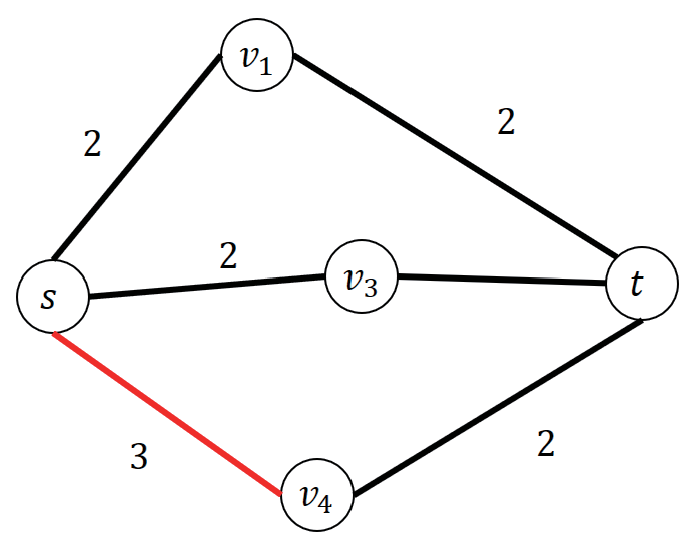
\includegraphics[width=0.7\textwidth]{figures/1.eps}\\
  \caption{Instance}\label{q4_1}
\end{figure}

As is shown in Fig~\ref{q4_1}, there are $k$ paths from $x$ to $y$. If there is none of the paths from $y$ to $z$, which jointed with those from $x$ to $y$, then the result is true trivially.

If there are one path from $y$ to $z$ that joint a path from $x$ from $y$, then we can see that there will appear another path that from $x$ to $z$ without via $y$. It does not decrease the quantity of paths of the trivial case.

Consider a more general case, as is shown in Fig~\ref{q4_2}, when there is a path from $y$ to $z$ that joint with $q$ paths from $x$ to $y$. We can see that this path from $y$ to $z$ can be excluded because there is already a path from $x$ to $z$ without via $y$.
\begin{figure}[H]
  \centering
  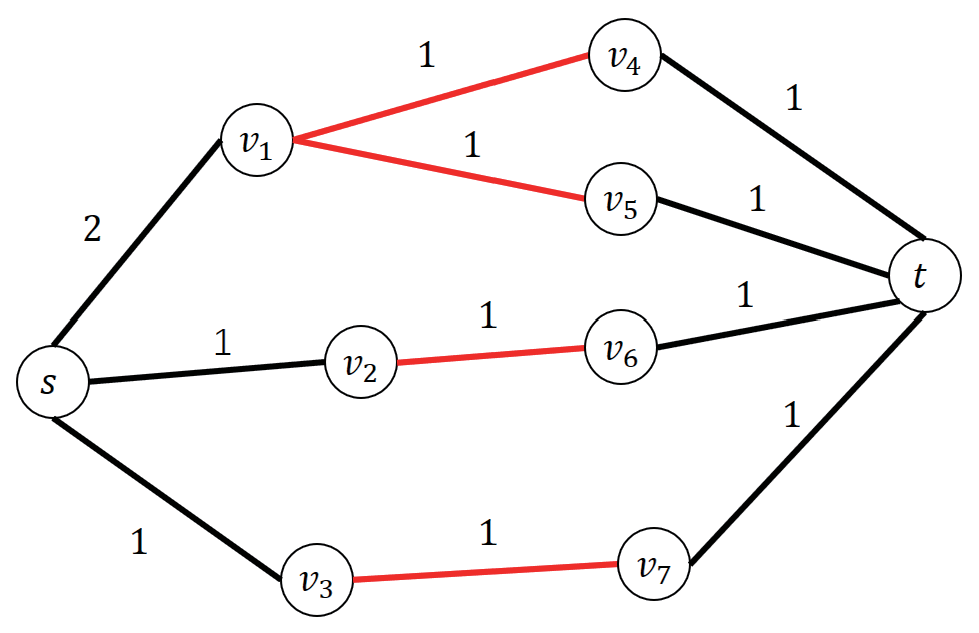
\includegraphics[width=0.7\textwidth]{figures/2.eps}\\
  \caption{Instance}\label{q4_2}
\end{figure}

Now consider the general case, as is shown in Fig~\ref{q4_3},when there is $t$ paths from $y$ to $z$, all of which joint with $q$ paths from $x$ to $y$. We
can see that these $t$ paths make sure that the sub path joint with the $q$ paths from $x$ to $y$ disjoint. We reconstruct the path by choosing $x\to x_{q1}\to x_{q2}\to x_{q3}...\to x_{qu}\to ... \to z$, $x\to x_{q-1\;1}\to x_{q-1\;2}\to x_{q-1\;3}...\to x_{q-1\;f}\to x_{qg} \to ... \to z$ ... $x\to x_{11}\to x_{12}\to x_{13}...\to x_{1h}\to x_{2o}\to ... \to z$. It is obviously that the quantity paths will not decrease. 
\begin{figure}[H]
  \centering
  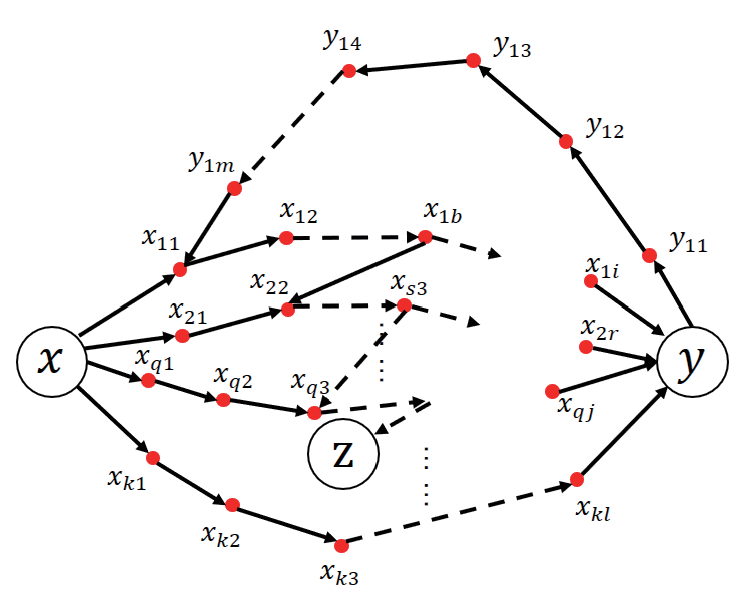
\includegraphics[width=0.7\textwidth]{figures/3.eps}\\
  \caption{Instance}\label{q4_3}
\end{figure}
Therefore the conclusion is ``Yes".











